% Session 8 -- the parton construction: an enlarged local Hilbert space, cut back down
% Placement: sec. "The parton construction", after the single-occupancy constraint (8.11).
% Rendered by figures/blender/s08f04_parton.py, labels in figures/overlays/s08f04_parton.tex.
\begin{aqmfigure}{fig:s08:parton}{What the Abrikosov-fermion rewriting (8.10) costs, and what it
gives us. (a) The four fermionic states of a site. The two singly-occupied states give the physical
spin-$1/2$ doublet exactly. The empty and doubly-occupied states, drawn as ghosts with a cross, are
extra unphysical states, which (8.10) maps to $\mathbf S_i=\mathbf 0$ and which the constraint
(8.11) removes by hand, and this constraint is the operator version of the Gutzwiller projector
(8.7). (b) What remains after the mean-field decoupling (8.14), which is an ordinary tight-binding
problem (8.15) for fermions with spin-$1/2$ and no charge, which hop with the self-consistent bond
amplitude $\chi_{ij}$, drawn as the thickness of the bond, here with two values for illustration.
Since there is one fermion per site, the resulting spinon model must be studied at half filling.
Taking the same $\chi_{ij}$ for both spin species keeps $\langle\mathbf S_i\rangle=\mathbf 0$, so
this mean field, unlike the magnetic mean fields of sessions 1 and 6, does not break time-reversal
symmetry.}
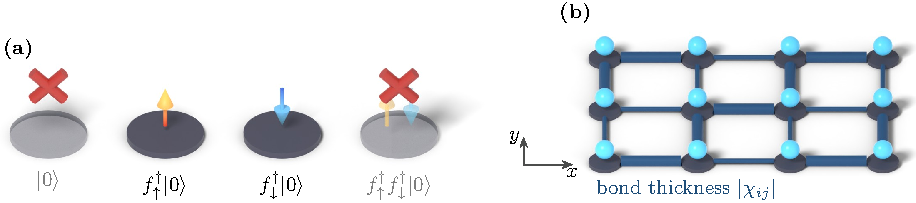
\includegraphics{figures/pdf/s08f04_parton.pdf}
\end{aqmfigure}
